\chapter{Evaluation}
\label{ch:evaluation}
To evaluate the proposed solution, firstly, it was tested against standard test cases, secondly, it was compared against XTurtle framework, lastly, it was validate with arbitrary large RDF files. This chapter discusses all of such details in the following text. 
\section{Experiment(1): Validating with RDF Suite Test}
The evaluation phase finds its starting point at \citealp{TurtleTests:Online} where Test Suite files of Turtle serialization are found. Any new parser (focused on the same RDF serialization) can its proficiency be validated against these files. Files at \citealp{TurtleTests:Online} are recommended by W3 Consortium\footnote{\href{https://www.w3.org/}{W3 Consortium}} to validate a parser that parses a Turtle format.  

For evaluation, the precision and recall are computed using the equations \ref{eq:1} and \ref{eq:2} respectively.  
\begin{align} 
   Precision=  \frac{t_p}{t_p+f_p} \label{eq:1}
\end{align}
\begin{align}
   Recall =  \frac{t_p}{t_p+f_n} \label{eq:2}
\end{align}

\section{Experiment(2): Random Syntax Errors Generation}
In this experiment, number of syntax errors are arbitrarily created using a Poisson Distribution, for example. a user who is working on on RDF data for 8 hours and each one hour he is making a change (insert/modify/delete a text) is simulated. The average number of making syntax errors per time interval is represented by the parameter $\lambda$ . To make more clear, if   $\lambda$ = 5, it means that five syntax errors were occurred per hour.  Assuming a user can introduce 10 syntax error per hour

	\begin{figure}[ht]
	\begin{center}
		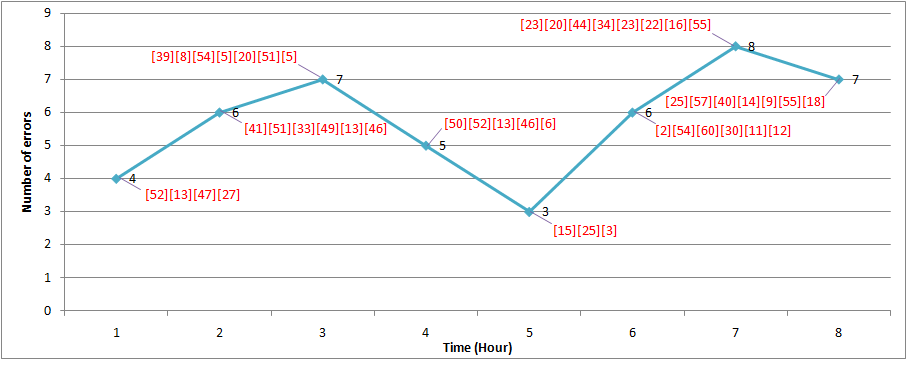
\includegraphics[scale=0.58,angle=0]{images/experiment2.png}
				\setlength\belowcaptionskip{-7mm}
		\caption{\textbf{Random Syntax Errors Distribution.} Number and types of syntax errors between brackets for a user in an interval of 8 hours. A Possion distribution with $\lambda$ = 5 models an average of 5 syntax errors per hour. A uniform distribution is computed to represent the type of errors} 
		\label{Fig:experiment2}
	\end{center}
\end{figure}
\section{Experiment(3): Impact of Numbers of Errors and RDF Volume on Performance }
To evaluate the performance of the proposed solution, this experiment will be held where number of syntax errors and RDF input data are varied. Two types of anthologies are used: small and medium size ones.  
%\section{Accuracy}

%\section{Scalability}








